\documentclass[times, 10pt,onecolumn]{article} 
\usepackage{latex8}
\usepackage{times}
\usepackage{url}
\usepackage{graphicx}
%\usepackage{amsfonts, amsthm}

\title{Symbolic Execution in Software Testing}
\author{
Xusheng Xiao\\
\small{xxiao2@ncsu.edu}\\
\and
Xi Ge\\
\small{xge@ncsu.edu}\\
\and
Da Young Lee\\
\small{dlee10@ncsu.edu}
}
\date{March 10, 2010}


\newcommand{\N}{\mathbb{N}}
\newcommand{\Z}{\mathbb{Z}}
\newcommand{\R}{\mathbb{R}}

\begin{document}
\maketitle
\thispagestyle{empty}
\pagestyle{empty}

\begin{abstract}
Symbolic execution is a way to track programs symbolicly rather than executing them with actual input value. With the impressive progress in constraint solvers, concolic path-based testing tools have literally blossomed up by combining both concrete and symbolic execution, which makes it possible to perform automatic path-based testing on large scale programs. However, these technologies are still suffering from the path explosion problem, since achieving 100\% path coverage is to enumerate all paths between two nodes in a graph, which is well known as a NP-hard problem. To alleviate this path explosion problem and to reduce the computation complexity, different techniques has been proposed, such as pruning search space of symbolic execution, selective symbolic execution and fitness-guided path exploration. In this report, we provide the details on the problem of test data generation and present three techniques to alleviate this path explosion problem. We also discuss the early researchers who contributed to the field of research of test data generation using symbolic execution. \end{abstract}
\section{Introduction} 
Symbolic execution~\cite{symbolic} is a way to track programs symbolicly rather than executing them with actual input value. Concolic path-based testing tools have literally blossomed up recently \cite{extenjpf,structural,mixed,exe,fuzzing,pex} with the impressive progress in constraint solvers. Concolic path-based testing tools combine both concrete and symbolic execution (referred as concolic execution~\cite{dart,cute} or mixed execution~\cite{mixed}), which makes it possible to perform automatic path-based testing on large scale programs. By executing the program under test with concrete values while performing symbolic execution, symbolic constraints on the inputs can be collected from the predicates in branch statements, forming an expression, called path condition. To explore new paths, part of the constraints in the collected path conditions are negated to obtain new path conditions, which are sent to a constraint solver to compute test inputs for new paths. In theory, all feasible execution paths will be exercised eventually through the iterations of constraint collection and constraint solving in DSE.

Whitebox fuzzing~\cite{fuzzing} executes the program under test with an initial, well-structured input, both concretely and symbolically. Along the execution, symbolic execution collects constraints on program inputs from the predicates in the conditional statements. The conjunction of these constraints of a execution path form an expression, called path condition. Satisfying the negation of each constraint in the path condition defines new inputs that exercise different control paths. Whitebox fuzzing repeats this process for the newly created inputs, with the goal of exercising many different control paths of the program under test and finding defects as fast as possible using various search heuristics. In practice, the search is usually incomplete because the number of feasible control paths grows exponentially with number of conditional statements in the program under test and because the precision of symbolic execution, constraint generation and solving is inherently limited. However, whitebox fuzzing has been shown to be very effective in finding new security vulnerabilities in several applications.

Hampi \cite{hampi} is designed and implemented as a constraint solver for string-manipulating programs. Hampi constraints express membership by regular language, fixed size context-free language. It may contain a fixed size string variable, context-free language definition, regular language definition and operations, and language-membership predicates. Given a set of string constraints over a string variable, Hampi outputs a string that satisfies all the constraints or reports that the constraints are unsatisfiable. Hampi is used as a component in testing, analysis, and verification applcations. Hampi can also be used to solve the intersection, containment, and equivalence problems for regular and fixed size context free languages.

CESE \cite{CESE} is an approach that targets at generating test inputs for programs accepting inputs, whose language can be described using context-free grammars. In particular, CESE is a hybrid approach that combines the advantages of two different approaches: specification-based enumerative test generation \cite{yagg} and dynamic symbolic execution \cite{system,symbolic,Test,counter,random}. CESE proposes symbolic grammar, which are in the form of context-free grammars. Symbolic grammar includes symbolic variables for terminals instead of actual concrete values, which are generally described using regular expressions. CESE automatically generates concrete values for symbolic variables in symbolic grammar by exploring the program under test using dynamic-symbolic-execution-based approaches. The primary advantage of symbolic grammars is that they reduce the state-space of possible values for inputs significantly.


\section{Pruning Search Space of Symbolic Execution}
Recent and impressive progress in constraint solvers as well as the combination of both concrete and symbolic execution (referred as concolic execution~\cite{cute,compositional} or mixed execution~\cite{mixed}) make it possible to perform automatic path-based testing on large scale programs. However, these technologies are still suffering from two major bottlenecks: efficient constraint solving and the path explosion phenomenon. S\'{e}bastien Bardin and Philippe Herrmann~\cite{prune} focus on the second issue and propose three complementary heuristics geared toward lowering path explosion. All these heuristics deal with different distinct sources of path explosion. 

To cover all paths of a program is not the primarily objective of current testing practices. Often the case, it is only required to fully cover a class of structural artifacts of the program code source, such as statements, branches or atomic predicates. In the rest of the section, we denote these three classes of artifacts as structural coverage. There is an obvious mismatch between path-based approaches and such item coverage goals: while each new test data does cover a new path, it may hit no new item. Thus, path-based testing methods tend to waste a lot of time trying to compute irrelevant test data, i.e. test data exercising no new structural coverage. 


To address the path explosion issue in path-based testing with item coverage objectives, they provide three heuristics to discard irrelevant paths as much as possible, reducing of the number of solver calls and the whole computation time. The three heuristics are used as enhancements of a (bounded) depth-first search (DFS) path-based procedure, either purely symbolic or concolic. Original path-based testing techniques were based on DFS~\cite{dart,cute, onthefly}, while some recent works advocate using other search strategies~\cite{exe,hybrid,fuzz}.

\subsection{Look-Ahead heuristic}
\begin{figure}
\centering
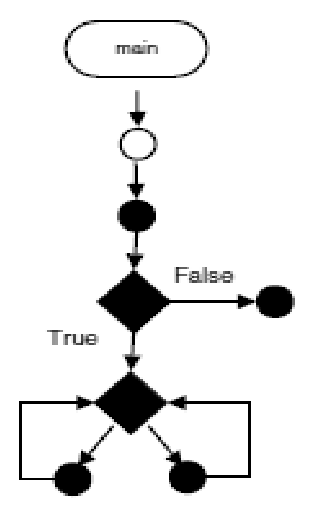
\includegraphics[scale=0.35,clip]{fig/la.eps} 
\caption{\label{fig:la}Example of Look-Ahead (LA) Heuristic} 
\end{figure}

The key idea of the Look-Ahead (LA) heuristic is to perform a reachability analysis in terms of reachable items in the CFG, and decide whether the current
path must be expanded based on the reachability analysis. If no new items can be reached, then exploration along the current path is stopped.

Figure \ref{fig:la} shows an example for illustrating the Look-Ahead (LA) heuristic. Let us assume the depth bound $k \geq 4$ and the objective is to achieve full statement coverage, and every path of the program is feasible. Then the original DFS based produre needs to explore $\approx2^k$ paths to achieve full coverage (because of the two nested loops) while DFS+LA requires at most 3 paths: one path to cover the false branch and two paths to cover two loops.

\subsection{Max-CallDepth (MCD) heuristic}
The major source of path explosion is function calls, and especially nested function calls. It is more embarrassing when only the top-level function is of interest. For example, it may be the case that the procedure explores alternative (long) paths due to backtrack in deep callees while a simple backtrack at top-level would be sufficient. Example of figure \ref{fig:mcd} gives such a behaviour.

\begin{figure}
\centering
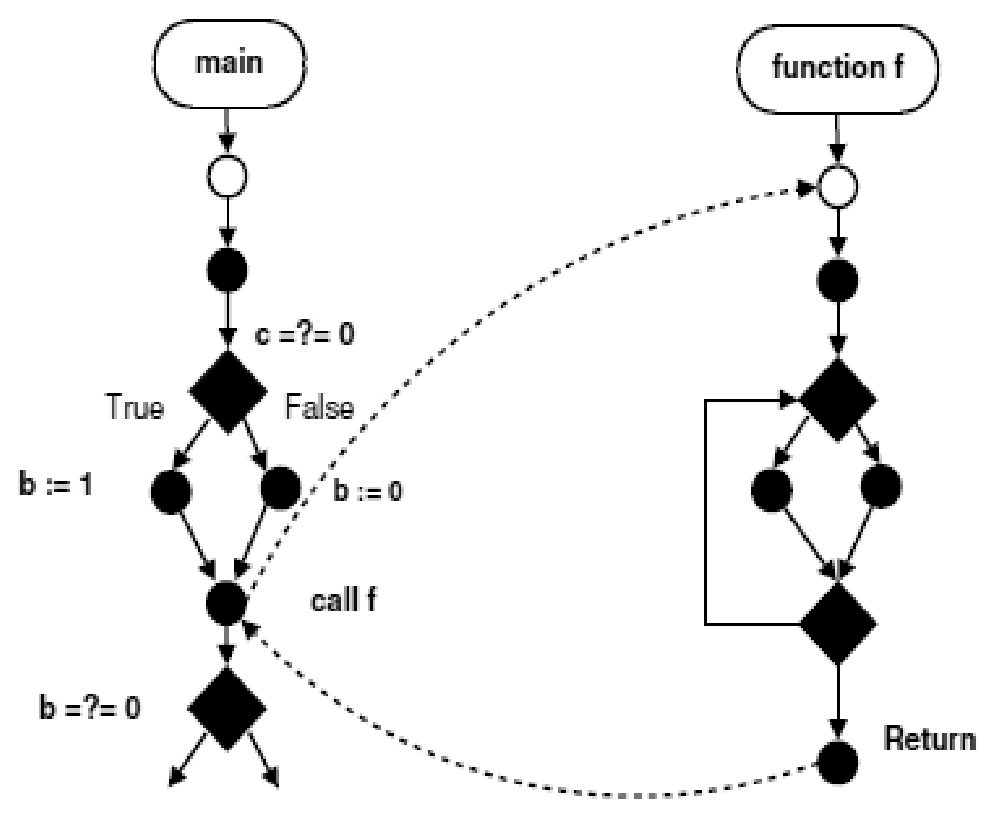
\includegraphics[scale=0.35,clip]{fig/mcd.eps} 
\caption{\label{fig:mcd}Example of Max-CallDepth (MCD) heuristic} 
\end{figure}

The principle of the Max-CallDepth heuristic (MCD) is to prevent backtracking in deep nested calls, hoping such a deep decision is not mandatory to cover the function under test. It is clear that this heuristic makes sense only in unit testing. Moreover, contrary to LA, MCD may discard relevant paths and prevent the full coverage of the function under test. On the other hand, on some programs MCD can discard many paths and still achieve full coverage. These results are summarised in the next property.

\subsection{Solve-First (SF) heuristic}




\section{Fitness}
\indent Structural software testing aims at achieving full or high code coverage such as statement and branch coverage of the program under test. The problem of testing for finding bugs could be reduced to the problem of structural testing that achieves full code coverage. A certain defected area of the source code could be considered as a statement guarded by a condition on the input values. For example, the negation of the assertion condition will witness a bug.\\
\begin{figure}[b]
\centering
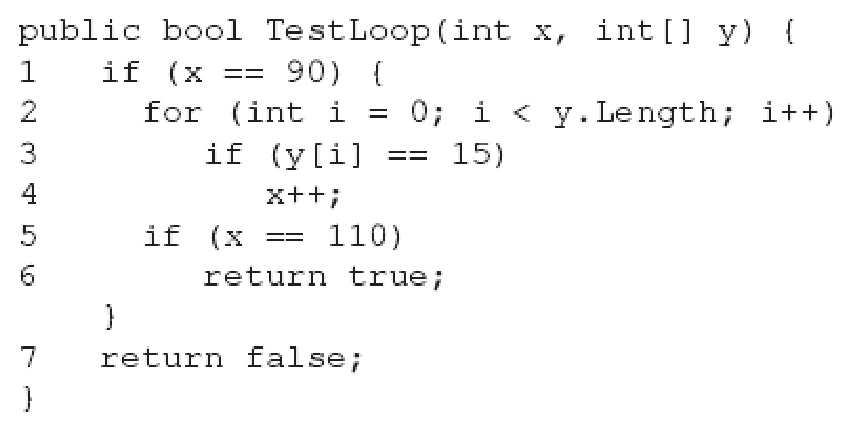
\includegraphics[scale=0.7]{fig/XiFitnessEPS.eps}
\caption{Figure 1. An example method under test.}
\end{figure}
\indent Random testing is one of the most commanly used technique for structural software testing since its easy implementation and the marginal overhead in choosing inputs. It simply generates the test input randomly and feed the input to the program under test. Even though the unbiased and effiecient nature of random testing, it will face difficulty to cover a certain statement or branch whose execution requires strict conditions on the input. For example, to cover the statement in line 6 of the example method in figure 1, the integer value of x needs to be exact 90, and the array of y contains more than 110 elements whose value are 15. This harsh condition on the input values makes it almost impossible to reach the statement in line 6.\\
\indent To address this issue faced by the random testing, dynamic symbolic execution(DSE) that systematically explores feasible paths of the program under test has been proposed recently. DSE executes the program for a given input, and performs collection of symbolic constraints on the inputs implied by predicate statements along the execution. The conjunction of all the conditions will be called path condition. DSE increases the code coverage by iteratively flipping the branch node of an already explored path and using constraint solver to generate test inputs based on the new path condition if it is satisfiable. For example, assuming the initial argument of x and y in the example method are 0 and \{0\}, respectively, the false branch of the line 1 statement, x!=90, is taken. Negating the branch will give the input value x=90 and y=\{0\} to cover the true branch of line 1. \\
\indent Even though DSE greatly improves the efficiency of achiving higher code coverage. It still faces multiple challenges in practical use. The covering of the true branch of line 5 needs exactly 20 executions of the true statement of line 3 inside the loop. By using DSE to hunt such a case, we would explore at least $2^{20}$ different execution paths before we can reach line 6 (using random searching strategy). This is in NP-Hard that renders the full coverage of the method almost impossible. 
\indent There are several other type of searching strategies besides random searching. DART and CUTE adoped the depth-first searching strategy and EXE provide either depth-first search strategy and the mixture of best-first and depth-first strategy based on the code coverage heuristics. A generational search that explores only a very limited horizon are usd by SAGE.The drawbacks of all the searching strategies are biased nature that favor particular control flow points, e.g, the depth-first searching favors the final branches and the width-first searching strategy favors the first branches. None of these ways are capable of reaching target test stated in the example method efficientlly.\\
\indent To enhance the efficiency of DSE in achieving higher code coverage, the authors has proposed a novel way to guide DSE called fitnex, which is a searching strategy that uses state-dependent fitness values to guide path exploration. Through the fitness-guided path exploration, the full code coverage in cases like the example method under test will be more easily achieved. The procedure to use Fitnex strategy on the example method showed in figure 1 will be presented as follows:
\indent \textbf{Fitness computation for a path.} The fitness values are used to decide which branch's flipping would be more helpful in covering the target statement. Extracted from predicate of the conditions in executing test target, fitness functions are used to compute the fitness value, reflecting how close a path's execution is to the covering of the test target. The exploration then honors the fittest path which is the closest to the covering of the test target. The fitness function for the example method is $f(x)=|110-x|$. The smaller the fitness function value, the closer the path's execution is to cover the target. Considering the following 5 execution path,\\ 
\begin{center}
\begin{tabular}{|c|c|c|}\hline
Test & procedure & Path \\\hline
0 & TestLoop(0, new int[] {0}); & Path 0: 1F\\\hline
1 & TestLoop(90, new int[] {0}); & Path 1: 1T, 2T, 3F, 2F, 5F\\\hline
2 & TestLoop(90, new int[] {15}); &Path 2: 1T, 2T, 3T, 2F, 5F\\\hline
3 & TestLoop(90, new int[] {15, 0}); & Path 3: 1T, 2T, 3T, 2T, 3F, 2F, 5F\\\hline
4 & TestLoop(90, new int[] {15, 15});& Path 4: 1T, 2T, 3T, 2T, 3T, 2F, 5F\\\hline
\end{tabular}\\
Form 1. Several explored paths
\end{center}
Their fitness values for these paths are NA (for that the target test is not even reached), 20($|110 - 90|$), 19($|110 - 91|$), 19($|110 - 91|$), and 18(|110 - 92|) respectively. According to the proposed algorithm, the path 4 will be prefered since it the smallest value among all the paths which means that Path 4 is the closest path to the target test. Using symbolic value to compare fitness values may not to be a good idea since the comparison between symbolic values is quite expensive due to the invoking of constraint solver and the pairwise comparison is needed. Therefore, the concrete values are computed and compared. In general,  the predicate can be used to generate fitness functions to calculate how close a execution path to target test. The follwing form shows several instances, column 1 shows the predicate of the target test, column 2 shows the fitness function derived from it.\\
\begin{center}
\begin{tabular}{|c|c|}\hline
Predicate & Fitness function \\\hline
$F(a==b)$ & $|a-b|$ \\\hline
$F(a>b)$ & $(b-a)+k$ \\\hline
$F(a>=b)$ & $(b-a)$ \\\hline
$F(a<b)$ & $(a-b)+k$ \\\hline
$F(a<=b)$ & $(a-b)$ \\\hline
\end{tabular}\\
Form 2. Predicates and fitness function.
\end{center}
Besides the kind of predicates listed above, there is another category of target test that are guarded with boolean value rather than number value. In that case, deriving the fitness function will be much harder and no strategy has been proposed.
\indent\textbf{Fitness-gain computation for a branch.} Selecting branch node in a path to flip in order to approach the target test could be reduced to selecting a branch node that (1)has at least one new branch that has not been covered yet,(2)has the best potential to improve the fitness value of the current path. The fitness gain is defined as the decreasement of the fitness value before and after the flipping of a branch. The fitness gain could be used to prioritize the flipping of various branches. For example, the fitness-gain of flipping the branch in line 3 for path 1 is 1; The flipping of same branch in Path 3 will result in fitness-gain of same degree. Intuitively, not all the flipping will result in desirable fitness-gain. For example, the flip from true to false of line 3 in path 3 will cause the fitness-gain of -1.\\
\indent Each branch b in a path p is assigned a composite number $F(p)-FGain(b)$, whare $F(p)$ is the fitness value of the path p, and $FGain(b)$ is the fitness-gain of the flipping b in p. Then the priority of the flips all over the explored paths could be decided according to the composite value. Consider the previous four tests as a example, the smallest composite value comes at flipping the false branch in line 2 of the path 4 since the node has the least composite value 17. For several iterations, the strategy will eventually achieve the path whose fitness value is exactly 0, in another word, reach the target test.


\input{selective}

\section{Major Contributors}
The concept of symbolic execution was introduced academically with descriptions of the Select system, proposed by Boyer et al~\cite{select}. In 1976, test data generation using symbolic execution was first proposed by James C. King~\cite{symbolic}. Around the same time, Clarke also did the work on this~\cite{test76}. Their pioneer works open the ways to automatic test data generation by using symbolic execution to do static analysis of code for path safety and prove theorems about code. However, these static ways faced the exponential state space explosion problem, which made it only practical for small programs. In recent years, Koushik Sen, whose paper on concolic testing~\cite{dart} won the ACM SIGSOFT Distinguished Paper Award at ESEC/FSE '05, proposed CUTE and DART tools, blossoming up the path-based automatic test data generation using symbolic execution. With the impressive progress of constraint solvers and concolic path-based testing~\cite{extenjpf,structural,mixed,exe,fuzz,pex}, it is possible to perform automatic path-based testing on large scale programs. Pex~\cite{pex}, a symbolic execution test generation tool for .NET proposed by Nikolai Tillmann, has been used to test .NET core libraries and found serious bugs. To alleviate the classic path explosion problem, many new techniques are also been proposed by Xie~\cite{fitness}, Godefroid~\cite{compositional} and so on.


\bibliographystyle{plain}
\bibliography{references}
\end{document}